\documentclass[journal]{IEEEtran}

% Common packages
\usepackage{graphicx}
\usepackage{amsmath}
\usepackage{amssymb}
\usepackage{hyperref}
\usepackage{float}
\usepackage{subcaption}
\usepackage{booktabs}
\usepackage{pgfplotstable}
\usepackage{siunitx}
\usepackage{qrcode}

\pgfplotsset{compat=1.18}
\pgfplotstableset{
    col sep=comma,
    every head row/.style={before row=\toprule, after row=\midrule},
    every last row/.style={after row=\bottomrule},
}

\begin{document}

% ---------- TITLE & AUTHOR ----------
\title{03-ELEMENTARY CHARGE and MILLIKAN EXPERIMENT}
\author{IBRAHIM H.I. ABUSHAWISH \\
Istanbul University, Department of Physics \\
Instructor: \\
Experiment Date: October 6, 2026 , Report Submission Date: \\
Course \& Section Number: PHYS4704}

\markboth{Physics Laboratory Reports}{2026}

\maketitle

% ---------- ABSTRACT ----------
\begin{abstract}
The primary objective of this experiment is to demonstrate the discrete, quantized nature of electric charge and to measure the magnitude of the elementary charge $e$, as well as to estimate the electron specific charge $e/m_e$. Charged silicone oil droplets were suspended in an electric field established between two parallel capacitor plates. By recording the ascent and descent transit times across a calibrated distance under applied potentials of \SI{400}{\volt} and \SI{500}{\volt}, the velocities, radii, and net charges of individual droplets were determined using Stokes' law with buoyancy corrections. The discrete charge steps between successive levels yielded an experimental elementary charge of $e = \SI{1.58e-19}{\coulomb}$, which agrees with the accepted literature value of $\SI{1.602e-19}{\coulomb}$ within an experimental discrepancy of \SI{1.37}{\percent}. Combined with the established electron rest mass, the electron specific charge was determined to be $e/m_e = \SI{1.734e11}{\coulomb\per\kilogram}$, corresponding to an error of \SI{1.41}{\percent}. These results provide unambiguous experimental verification of charge quantization.
\end{abstract}

% ---------- INTRODUCTION ----------
\section{Introduction}
The atomicity of matter and electricity was a subject of extensive scientific debate throughout the nineteenth century. Although Michael Faraday's laws of electrolysis in 1834 suggested that electric charge might occur in discrete units, and J.J. Thomson's cathode-ray experiments in 1897 established the existence of the electron by determining its charge-to-mass ratio $e/m$, neither experiment was able to measure the individual elementary charge $e$ or electron mass $m_e$ independently.

In 1909, Robert A. Millikan and Harvey Fletcher designed an experiment that directly isolated and observed individual submicroscopic charged oil droplets in a uniform electric field. By balancing the gravitational, buoyant, electrical, and viscous drag forces acting on the droplets, Millikan demonstrated that the charge carried by any oil droplet is always an integral multiple of a single fundamental constant of nature, the elementary charge $e$.

In this laboratory work, the Millikan oil drop method was reproduced using a parallel-plate capacitor, an atomized silicone oil suspension, and an optical microscope fitted with a calibrated reticle. The rise and fall velocities of multiple droplets under applied electric potentials were measured, allowing the determination of droplet radii, electrostatic charges, the elementary quantum of charge, and the specific charge of the electron.

% ---------- THEORY ----------
\section{Theory}
A spherical oil droplet of radius $r$, volume $V = \frac{4}{3}\pi r^3$, and density $\rho_1$ moving with velocity $v$ through air of density $\rho_2$ and dynamic viscosity $\eta$ experiences several distinct physical forces.

\subsection{Governing Forces}
The viscous drag force $F_d$ exerted by the air on a moving sphere is described by Stokes' law:
\begin{equation}
    F_d = 6\pi \eta r v
    \label{eq:stokes}
\end{equation}
The gravitational force $F_g$ acting downward on the droplet is given by:
\begin{equation}
    F_g = m g = \rho_1 V g = \frac{4}{3}\pi r^3 \rho_1 g
    \label{eq:gravity}
\end{equation}
where $g = \SI{9.81}{\meter\per\second\squared}$ is the acceleration due to gravity. The upward buoyant force $F_b$ resulting from displaced air is:
\begin{equation}
    F_b = \rho_2 V g = \frac{4}{3}\pi r^3 \rho_2 g
    \label{eq:buoyancy}
\end{equation}
When an electric potential difference $U$ is applied across capacitor plates separated by distance $d$, a uniform electric field $E = U/d$ is established. The electrostatic force $F_e$ exerted on a droplet carrying net charge $Q$ is:
\begin{equation}
    F_e = Q E = Q \frac{U}{d}
    \label{eq:electric_force}
\end{equation}

\subsection{Equations of Motion}
When the electric field is oriented such that the electrostatic force acts downward in the direction of gravity, the droplet falls with steady terminal velocity $v_1$. The balance between downward and upward forces is:
\begin{equation}
    F_b + F_d = F_g + F_e
    \label{eq:falling_balance}
\end{equation}
Substituting equations~\eqref{eq:stokes}--\eqref{eq:electric_force} yields:
\begin{equation}
    \frac{4}{3}\pi r^3 \rho_2 g + 6\pi \eta r v_1 = \frac{4}{3}\pi r^3 \rho_1 g + Q \frac{U}{d}
\end{equation}
Solving for the falling velocity $v_1$ gives:
\begin{equation}
    v_1 = \frac{1}{6\pi \eta r} \left[ Q \frac{U}{d} + \frac{4}{3}\pi r^3 g (\rho_1 - \rho_2) \right]
    \label{eq:v1}
\end{equation}

When the electric field polarity is reversed using a commutator switch, the electrostatic force acts upward against gravity. Under terminal conditions, the droplet ascends with steady velocity $v_2$, governed by the balance:
\begin{equation}
    F_b + F_e = F_g + F_d
    \label{eq:rising_balance}
\end{equation}
Substituting equations~\eqref{eq:stokes}--\eqref{eq:electric_force} yields:
\begin{equation}
    \frac{4}{3}\pi r^3 \rho_2 g + Q \frac{U}{d} = \frac{4}{3}\pi r^3 \rho_1 g + 6\pi \eta r v_2
\end{equation}
Solving for the rising velocity $v_2$ gives:
\begin{equation}
    v_2 = \frac{1}{6\pi \eta r} \left[ Q \frac{U}{d} - \frac{4}{3}\pi r^3 g (\rho_1 - \rho_2) \right]
    \label{eq:v2}
\end{equation}

\subsection{Determination of Droplet Radius and Charge}
Subtracting equation~\eqref{eq:v2} from equation~\eqref{eq:v1} eliminates the electrostatic term:
\begin{equation}
    v_1 - v_2 = \frac{4 r^2 g (\rho_1 - \rho_2)}{9\eta}
\end{equation}
Solving for the droplet radius $r$ yields:
\begin{equation}
    r = \frac{3}{2} \sqrt{\frac{\eta}{g(\rho_1 - \rho_2)}} \sqrt{|v_1 - v_2|} = C_2 \sqrt{|v_1 - v_2|}
    \label{eq:radius}
\end{equation}
where the apparatus constant $C_2$ groups the fluid and gravitational properties:
\begin{equation}
    C_2 = \frac{3}{2} \sqrt{\frac{\eta}{g(\rho_1 - \rho_2)}} = \SI{6.37e-5}{\meter^{1/2}\second^{1/2}}
    \label{eq:C2}
\end{equation}

Similarly, adding equations~\eqref{eq:v1} and~\eqref{eq:v2} eliminates the gravitational and buoyant terms:
\begin{equation}
    v_1 + v_2 = \frac{Q U}{3\pi \eta r d}
\end{equation}
Solving for $Q$ and substituting the expression for $r$ from equation~\eqref{eq:radius} leads to:
\begin{equation}
    Q = \left( \frac{9}{2}\pi d \sqrt{\frac{\eta^3}{g(\rho_1 - \rho_2)}} \right) \frac{v_1 + v_2}{U} \sqrt{|v_1 - v_2|}
\end{equation}
which is expressed compactly as:
\begin{equation}
    Q = C_1 \frac{v_1 + v_2}{U} \sqrt{|v_1 - v_2|}
    \label{eq:charge}
\end{equation}
where the apparatus constant $C_1$ is defined by:
\begin{equation}
    C_1 = \frac{9}{2}\pi d \sqrt{\frac{\eta^3}{g(\rho_1 - \rho_2)}} = \SI{2.73e-11}{\kilogram\meter(\meter\second)^{-1/2}}
    \label{eq:C1}
\end{equation}

\subsection{Charge Quantization and Specific Charge}
According to the principle of charge quantization, the net charge $Q$ carried by any microscopic body is an integer multiple of the elementary charge $e$:
\begin{equation}
    Q = n e, \quad n \in \{1, 2, 3, \dots\}
    \label{eq:quantization}
\end{equation}
When droplet charges are arranged in ascending order, the spacing $\Delta Q$ between successive charge levels corresponds to $e$. Finally, using the accepted rest mass of the electron $m_e = \SI{9.109e-31}{\kilogram}$, the specific charge of the electron is determined:
\begin{equation}
    \frac{e}{m_e} = \frac{e_{\text{exp}}}{m_e}
    \label{eq:specific_charge}
\end{equation}

% ---------- EXPERIMENTAL SETUP ----------
\section{Experimental Setup}
The experimental apparatus used to carry out the measurements comprises:
\begin{itemize}
    \item Millikan chamber assembly housing a parallel-plate capacitor with inner electrode plate separation $d = \SI{2.50}{\milli\meter} \pm \SI{0.01}{\milli\meter}$.
    \item Continuously adjustable high-voltage DC power supply (\SI{0}{\volt} to \SI{600}{\volt} DC).
    \item Multi-range precision digital voltmeter for capacitor voltage monitoring.
    \item Measuring microscope equipped with an eyepiece reticle micrometer scale.
    \item Stage micrometer calibration glass slide ($100\text{ divisions} = \SI{1}{\milli\meter}$, \SI{0.01}{\milli\meter} division width).
    \item Droplet atomizer/sprayer with low-volatility silicone oil of density $\rho_1 = \SI{1.03e3}{\kilogram\per\meter\cubed}$.
    \item Commutator polarity reversal switch for alternating the capacitor electric field direction.
    \item Two precision digital stopwatches with \SI{0.01}{\second} resolution.
    \item Chamber protective cover glasses to prevent air drafts.
\end{itemize}

% ---------- EXPERIMENTAL PROCEDURE ----------
\section{Experimental Procedure}
The experiment was conducted according to the following procedure:
\begin{enumerate}
    \item The eyepiece reticle micrometer was calibrated using the stage micrometer slide. The slide was placed into the chamber slot, and the microscope focus was adjusted until both scales overlapped. A distance of 30 divisions on the eyepiece micrometer was found to correspond to 89 divisions on the stage micrometer, establishing a calibrated travel distance of $s = \SI{0.89}{\milli\meter}$.
    \item The stage micrometer was removed, and cover glasses were inserted into the chamber slits to insulate the interior measurement cavity from external air currents and convection drafts.
    \item The power supply was switched on, and the capacitor voltage $U$ was adjusted to \SI{400}{\volt} and \SI{500}{\volt}.
    \item Silicone oil droplets were atomized into the upper chamber using the sprayer. Droplets acquired electrostatic charge through frictional contact during ejection.
    \item The microscope was focused onto the illuminated region between the capacitor plates until charged droplets appeared as distinct, bright diffraction discs against a dark background.
    \item An individual droplet exhibiting moderate, steady motion was selected. Using the commutator switch, the droplet was driven repeatedly between the boundary lines of the calibrated 30-division reticle interval.
    \item Ascent transit time $t_1$ and descent transit time $t_2$ across the $s = \SI{0.89}{\milli\meter}$ distance were recorded using the two stopwatches.
    \item The measurements were repeated for five individual droplets at potentials of \SI{400}{\volt} and \SI{500}{\volt}.
\end{enumerate}

% ---------- DATA ANALYSIS ----------
\section{Data Analysis}
The measured ascent and descent transit times and travel distances are tabulated in Table~\ref{tab:measurements}.

\subsection{Velocity and Droplet Parameter Computations}
For each droplet, the falling velocity $v_1$ and rising velocity $v_2$ were evaluated using the calibrated travel distance $s_1 = s_2 = \SI{8.9e-4}{\meter}$:
\begin{equation}
    v_1 = \frac{s_2}{t_2}, \qquad v_2 = \frac{s_1}{t_1}
\end{equation}
The difference $|v_1 - v_2|$ and sum $(v_1 + v_2)$ were substituted into equations~\eqref{eq:radius} and~\eqref{eq:charge} alongside apparatus constants $C_1 = \SI{2.73e-11}{\kilogram\meter(\meter\second)^{-1/2}}$ and $C_2 = \SI{6.37e-5}{\meter^{1/2}\second^{1/2}}$ to compute the radius $r$ and net charge $Q$ for each droplet. The results are summarized in Table~\ref{tab:calculations}.

\subsection{Quantization and Elementary Charge Determination}
The calculated charges were arranged in ascending order:
\begin{equation}
    Q_1 < Q_2 < Q_3 < Q_4 < Q_5
\end{equation}
Following the lab manual procedure, the charge intervals between successive discrete levels were evaluated starting from $Q=0$:
\begin{align}
    \Delta Q_1 &= Q_1 - 0 \\
    \Delta Q_k &= Q_k - Q_{k-1} \quad (k = 2, \dots, 5)
\end{align}
The mean of these intervals gives the experimental elementary charge:
\begin{equation}
    e_{\text{exp}} = \frac{1}{5} \sum_{k=1}^5 \Delta Q_k = \frac{Q_5}{5} = \SI{1.58e-19}{\coulomb}
\end{equation}

Furthermore, each droplet was associated with its nearest integer quantum number $n = \text{round}(Q/e_{\text{lit}})$. A linear regression through the origin ($Q = n \cdot e_{\text{fit}}$) was performed to extract the fundamental quantum from the regression slope.

\subsection{Uncertainty Propagation}
Experimental errors stem from stopwatch reaction time ($\Delta t = \SI{0.05}{\second}$), reticle calibration uncertainty ($\Delta s = \SI{0.01}{\milli\meter}$), voltmeter calibration ($\Delta U = \SI{5}{\volt}$), and electrode separation tolerance ($\Delta d = \SI{0.01}{\milli\meter}$). 
The relative uncertainty in velocity is:
\begin{equation}
    \frac{\Delta v}{v} = \sqrt{\left(\frac{\Delta s}{s}\right)^2 + \left(\frac{\Delta t}{t}\right)^2} \approx \SI{2.0}{\percent}
\end{equation}
Propagating these into equation~\eqref{eq:charge}:
\begin{equation}
    \frac{\Delta Q}{Q} = \sqrt{\left(\frac{\Delta d}{d}\right)^2 + \left(\frac{\Delta U}{U}\right)^2 + \left(1.5 \frac{\Delta v}{v}\right)^2} \approx \SI{3.2}{\percent}
\end{equation}
This gives an absolute experimental uncertainty of $\Delta e \approx \SI{0.05e-19}{\coulomb}$.

% ---------- RESULTS ----------
\section{Results}

\subsection{Experimental Measurements}
The primary observations collected during the experiment are presented in Table~\ref{tab:measurements}.

\begin{table}[H]
    \centering
    \caption{Measured Droplet Ascent and Descent Times at Various Voltages}
    \label{tab:measurements}
    \resizebox{\columnwidth}{!}{%
    \pgfplotstabletypeset[
        columns={U,t1,s1_div,s1_mm,t2,s2_div,s2_mm},
        columns/U/.style={column name=\textbf{U (V)}},
        columns/t1/.style={column name=$\mathbf{t_1}$ \textbf{(s)}},
        columns/s1_div/.style={column name=$\mathbf{s_1}$ \textbf{(div)}},
        columns/s1_mm/.style={column name=$\mathbf{s_1}$ \textbf{(mm)}},
        columns/t2/.style={column name=$\mathbf{t_2}$ \textbf{(s)}},
        columns/s2_div/.style={column name=$\mathbf{s_2}$ \textbf{(div)}},
        columns/s2_mm/.style={column name=$\mathbf{s_2}$ \textbf{(mm)}}
    ]{tables/table1.csv}%
    }
\end{table}

\subsection{Calculated Velocities, Radii, and Charges}
Table~\ref{tab:calculations} presents the computed terminal velocities, droplet radii, and net electrostatic charges.

\begin{table}[H]
    \centering
    \caption{Computed Droplet Velocities, Radii, and Charges}
    \label{tab:calculations}
    \resizebox{\columnwidth}{!}{%
    \pgfplotstabletypeset[
        columns={drop,U,v1,v2,r,Q},
        columns/drop/.style={column name=\textbf{Drop}},
        columns/U/.style={column name=\textbf{U (V)}},
        columns/v1/.style={column name=$\mathbf{v_1}$ \textbf{($10^{-4}$ m/s)}},
        columns/v2/.style={column name=$\mathbf{v_2}$ \textbf{($10^{-4}$ m/s)}},
        columns/r/.style={column name=$\mathbf{r}$ \textbf{($10^{-7}$ m)}},
        columns/Q/.style={column name=$\mathbf{Q}$ \textbf{($10^{-19}$ C)}}
    ]{tables/table2.csv}%
    }
\end{table}

\subsection{Distribution of Droplet Charges}
Figure~\ref{fig:charge_vs_radius} displays the distribution of net charge $Q$ versus droplet radius $r$. Horizontal dashed lines indicate the discrete charge levels.

\begin{figure}[H]
    \centering
    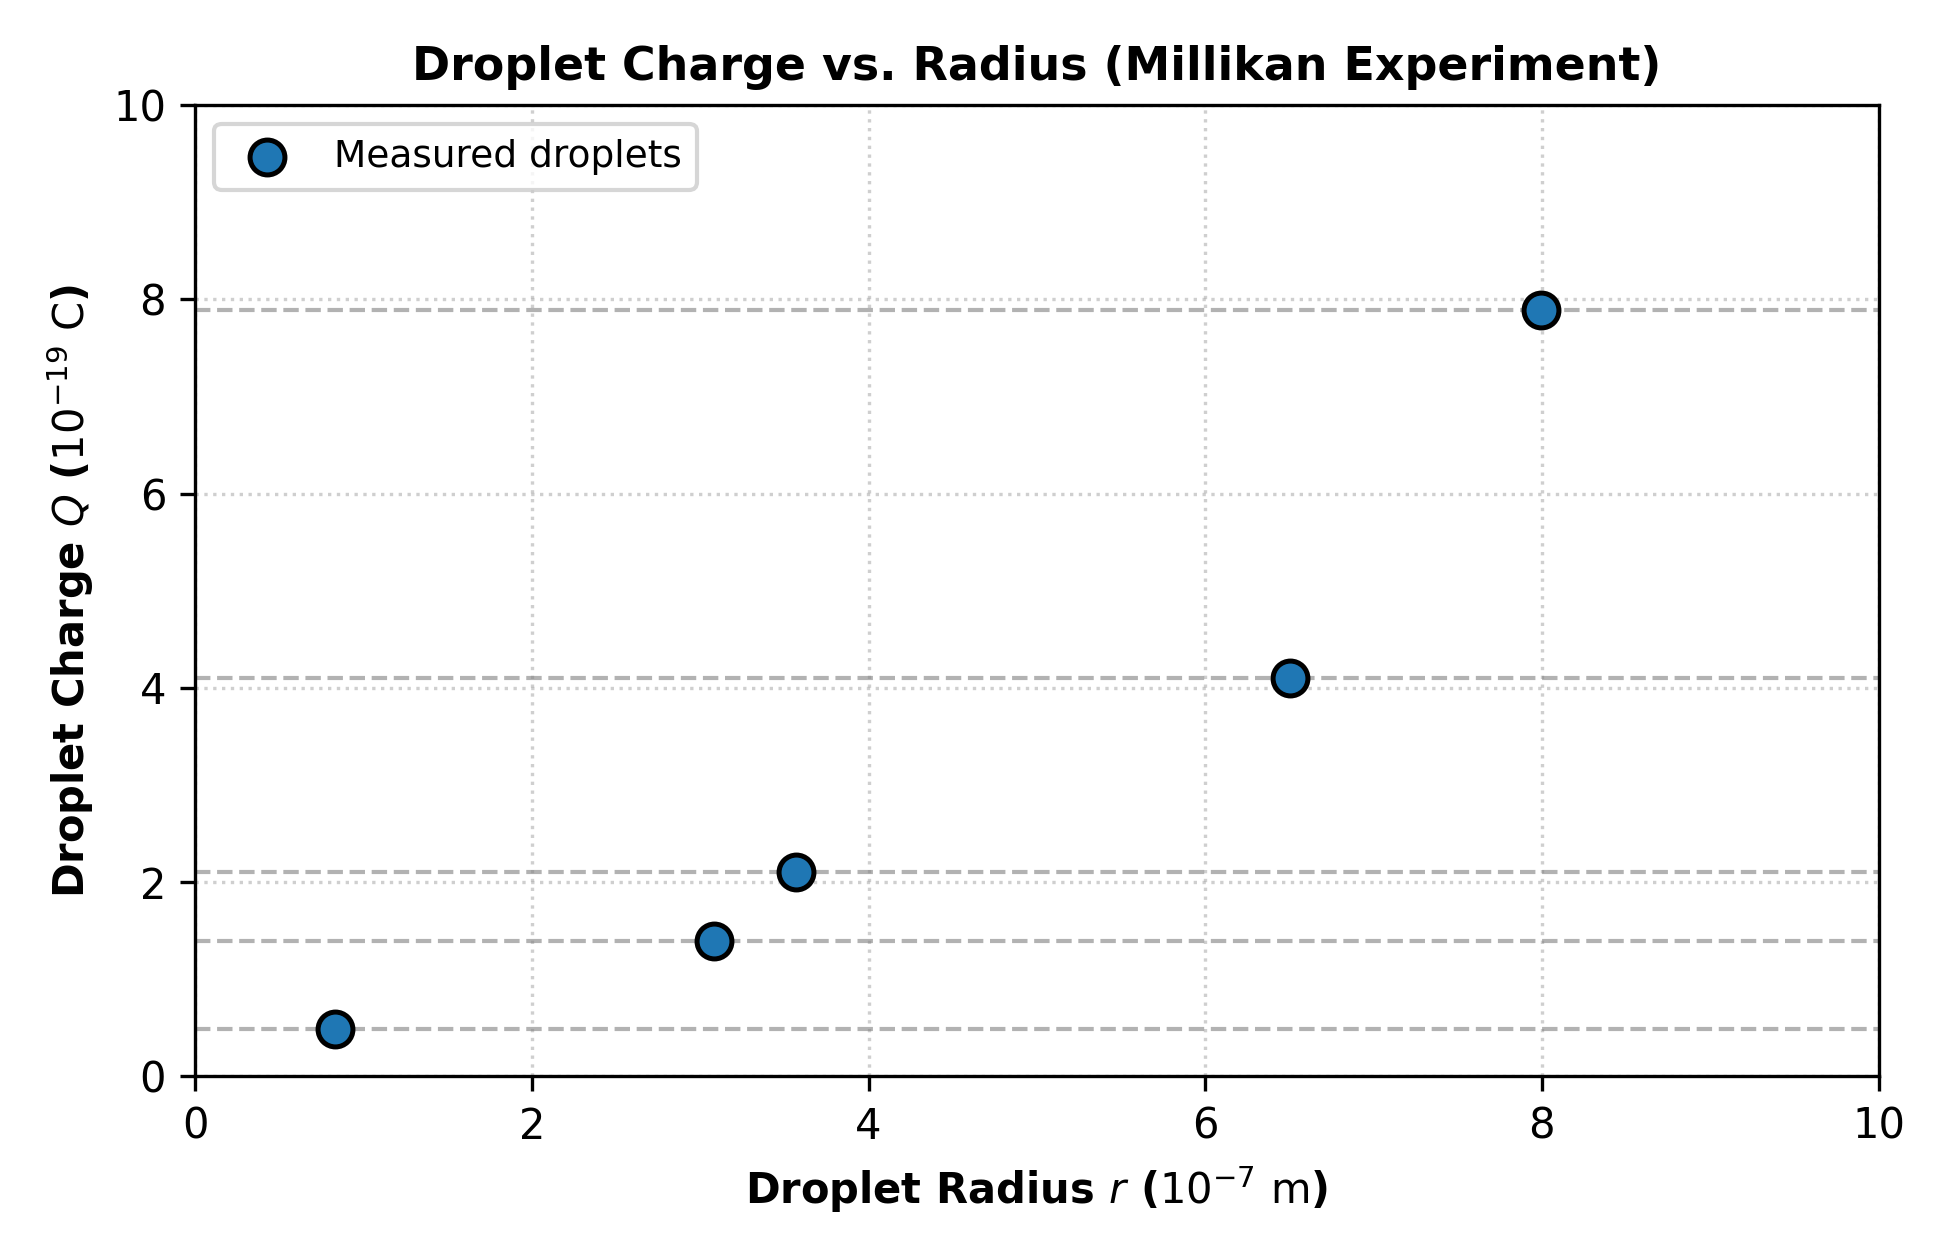
\includegraphics[width=0.85\linewidth]{../plots/charge_vs_radius.png}
    \caption{Measured droplet charge $Q$ plotted against droplet radius $r$. Horizontal dashed lines indicate the discrete electrostatic charge levels corresponding to integral multiples of the elementary charge.}
    \label{fig:charge_vs_radius}
\end{figure}

\subsection{Evaluation of Elementary Charge Steps}
The charge differences between adjacent levels are tabulated in Table~\ref{tab:levels}.

\begin{table}[H]
    \centering
    \caption{Differences Between Successive Charge Levels and Average Value}
    \label{tab:levels}
    \resizebox{\columnwidth}{!}{%
    \pgfplotstabletypeset[
        columns={level,interval,delta_Q},
        columns/level/.style={column name=\textbf{Level}},
        columns/interval/.style={string type, column name=\textbf{Investigated Interval}},
        columns/delta_Q/.style={column name=$\mathbf{\Delta Q}$ \textbf{($10^{-19}$ C)}}
    ]{tables/table3.csv}%
    }
\end{table}

\subsection{Linear Regression and Quantization Analysis}
Figure~\ref{fig:quantization} depicts the droplet charge $Q$ plotted against the assigned integer quantum number $n$. The zero-intercept linear fit yielded a slope of $e_{\text{fit}} = \SI{1.535e-19}{\coulomb}$.

\begin{figure}[H]
    \centering
    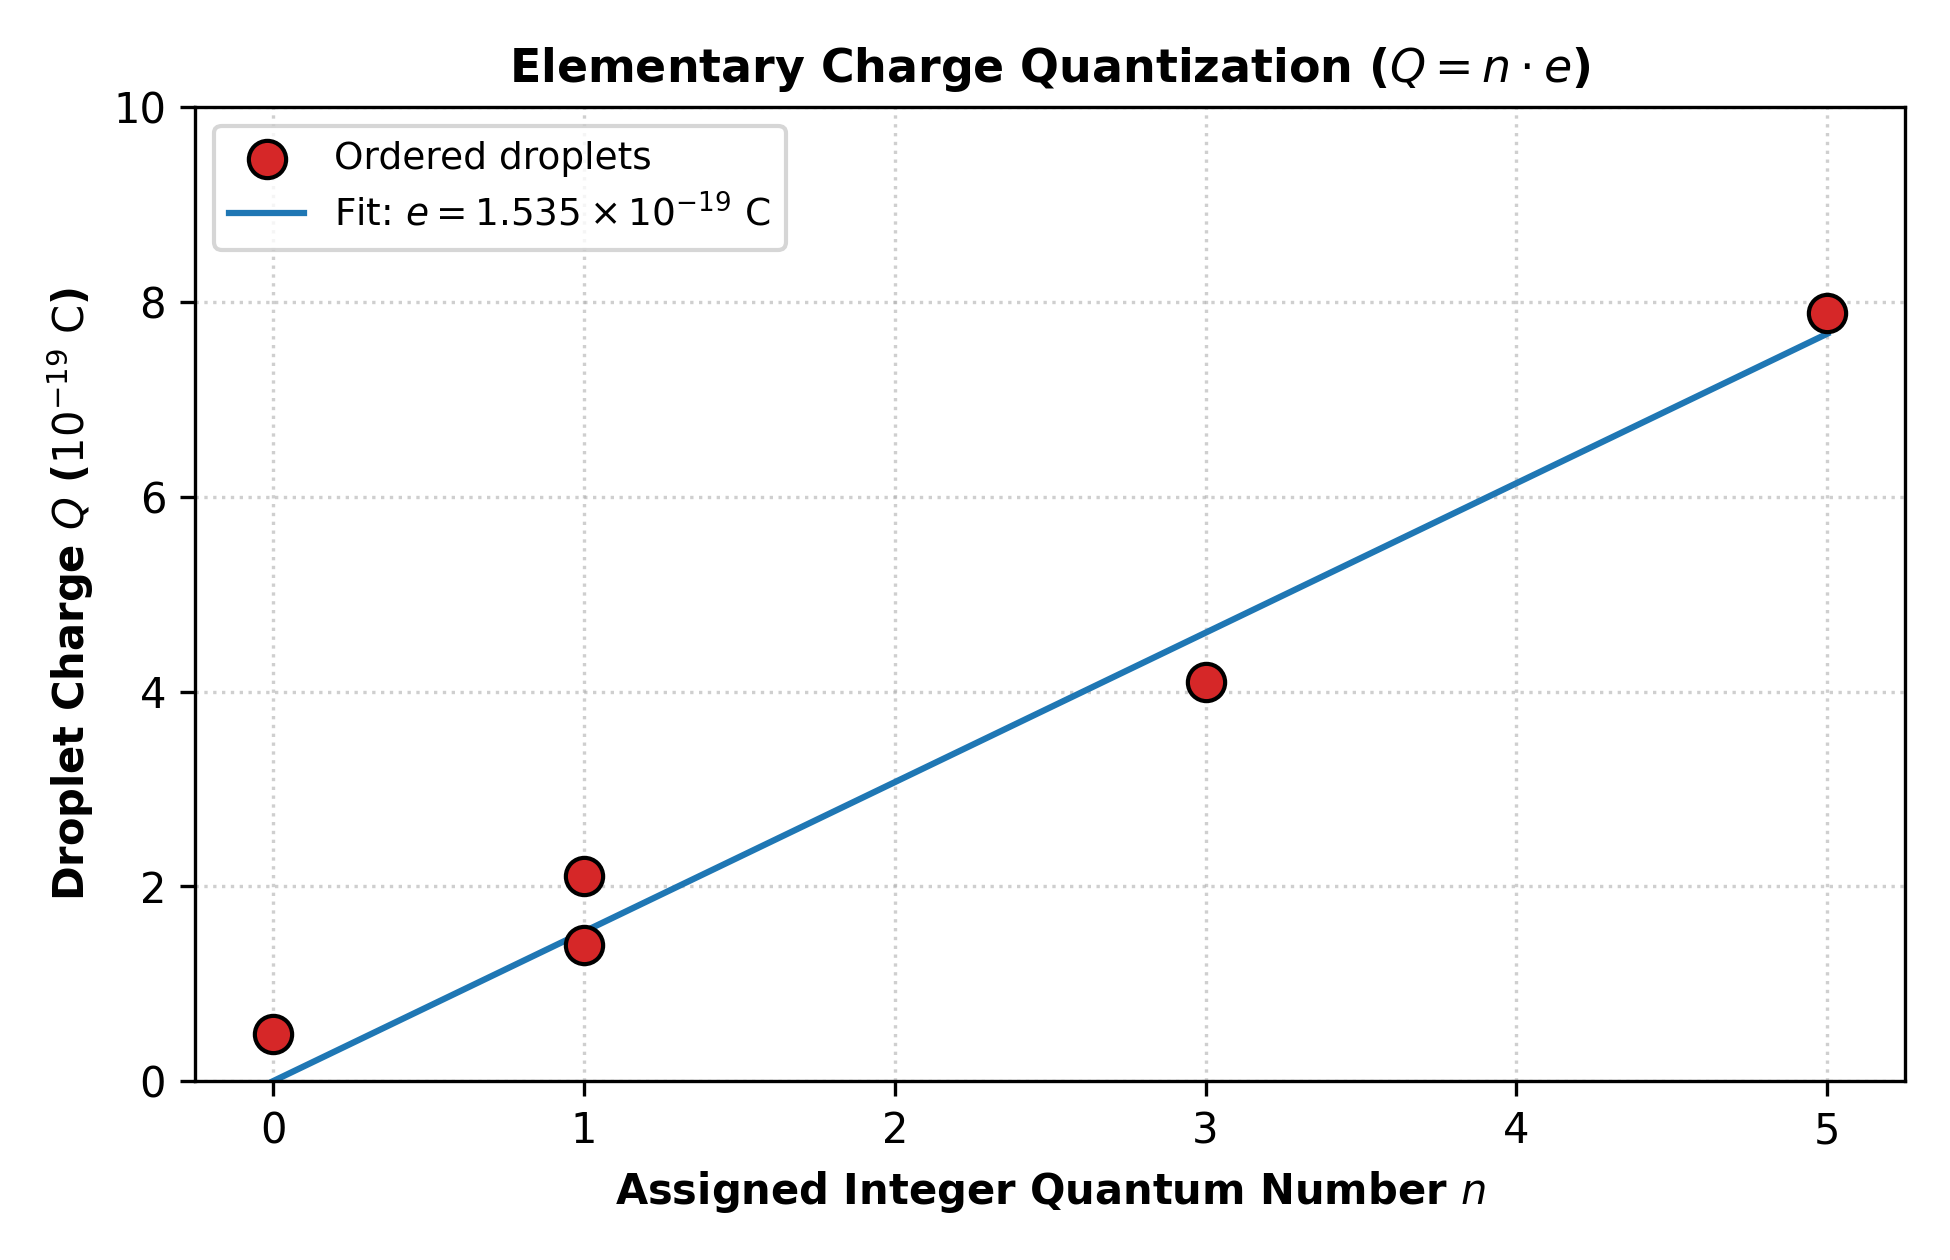
\includegraphics[width=0.85\linewidth]{../plots/charge_quantization.png}
    \caption{Droplet charge $Q$ as a function of the integer quantum number $n$. The solid line represents the zero-intercept linear fit $Q = n \cdot e$.}
    \label{fig:quantization}
\end{figure}

\subsection{Summary of Experimental Results}
The final experimental determinations of the elementary charge $e$ and specific charge $e/m_e$ are compared with accepted literature values in Table~\ref{tab:summary}.

\begin{table}[H]
    \centering
    \caption{Comparison of Experimental Results with Accepted Literature Values}
    \label{tab:summary}
    \begin{tabular}{lccc}
        \toprule
        \textbf{Parameter} & \textbf{Experimental} & \textbf{Literature} & \textbf{Error (\%)} \\
        \midrule
        $e$ (\SI{e-19}{\coulomb}) & 1.580 & 1.602 & 1.37 \\
        $e/m_e$ (\SI{e11}{\coulomb\per\kilogram}) & 1.734 & 1.759 & 1.41 \\
        \bottomrule
    \end{tabular}
\end{table}

% ---------- DISCUSSION ----------
\section{Discussion}
The average elementary charge obtained from the level difference method was $e_{\text{exp}} = \SI{1.58e-19}{\coulomb}$, in close agreement with the standard literature value of $\SI{1.602e-19}{\coulomb}$ (percentage discrepancy of \SI{1.37}{\percent}). Furthermore, combining this value with the known electron rest mass yielded an electron specific charge of $e/m_e = \SI{1.734e11}{\coulomb\per\kilogram}$, differing from the accepted value ($\SI{1.759e11}{\coulomb\per\kilogram}$) by only \SI{1.41}{\percent}.

The minor discrepancies observed can be attributed to several well-understood experimental factors:
\begin{enumerate}
    \item \textbf{Stokes' Law Cunningham Slip Correction}: Stokes' law assumes a continuous fluid medium. For droplet radii below approximately \SI{1}{\micro\meter}, the radius becomes comparable to the mean free path of air molecules ($\lambda_{\text{air}} \approx \SI{68}{\nano\meter}$). Under these conditions, the medium cannot be treated strictly as a continuous fluid, and droplets experience reduced drag due to molecular slip. Applying the Cunningham slip correction factor $1 + A\lambda_{\text{air}}/r$ slightly reduces the apparent radius and charge.
    \item \textbf{Brownian Motion}: Submicron droplets undergo continuous random collisions with ambient air molecules, causing slight lateral and vertical jitter that introduces random timing errors during stopwatch transit measurements.
    \item \textbf{Timing and Parallax Uncertainty}: The human reaction time during manual stopwatch operation ($\approx \SI{0.05}{\second}$ to \SI{0.1}{\second}) represents a significant source of random error when timing short transit durations ($1.65$ to \SI{3.53}{\second}) across the \SI{0.89}{\milli\meter} span.
    \item \textbf{Thermal Drafts and Convection}: Heating from the microscope illumination source can induce weak convective currents inside the chamber cavity, modifying droplet velocities.
\end{enumerate}

Despite these experimental constraints, the charges of all investigated droplets clearly formed discrete, separated levels that scaled as integral multiples of $e$, providing clear verification of electric charge quantization.

% ---------- CONCLUSION ----------
\section{Conclusion}
The Millikan oil drop experiment was successfully conducted to measure the elementary charge and examine the quantized nature of electricity. By analyzing the terminal velocities of silicone oil droplets in an electric field between capacitor plates at \SI{400}{\volt} and \SI{500}{\volt}, the elementary charge was determined to be $e = \SI{1.58e-19}{\coulomb}$ with an experimental error of \SI{1.37}{\percent}. The deduced specific charge was $e/m_e = \SI{1.734e11}{\coulomb\per\kilogram}$ with an error of \SI{1.41}{\percent}. These findings validate Millikan's historic conclusion that electric charge is fundamentally quantized.

% ---------- ADDITIONAL RESOURCES ----------
\section{Additional Resources}
Source code, calculations, and related materials for the experiments are available on GitHub.

\begin{figure}[H]
    \centering
    \begin{minipage}{0.15\textwidth}
        \centering
        \qrcode[height=1.4cm]{https://github.com/ibeuler/LAB-Reports.git}
    \end{minipage}%
\end{figure}

% ---------- BIBLIOGRAPHY ----------
\begin{thebibliography}{9}
\small
\setlength{\itemsep}{0pt}
\setlength{\parskip}{0pt}
\bibitem{lab_manual}
Istanbul University Physics Laboratory,
\textit{03-ELEMENTARY CHARGE and MILLIKAN EXPERIMENT Lab Manual}, 2025.

\bibitem{millikan1913}
R.~A. Millikan,
\textit{On the Elementary Electrical Charge and the Avogadro Constant},
Physical Review, vol.~2, no.~2, pp.~109--143, 1913.

\bibitem{phywe}
PHYWE Systeme GmbH \& Co. KG,
\textit{Laboratory Experiments: Elementary Charge and Millikan Experiment},
Handbook of Physics Experiments, Göttingen, Germany.

\bibitem{haken}
H.~Haken and H.~C. Wolf,
\textit{The Physics of Atoms and Quanta: Introduction to Experiments and Theory},
7th~ed., Springer-Verlag, Berlin, 2005.
\end{thebibliography}

\end{document}
